%\RequirePackage[l2tabu, orthodox]{nag}
\RequirePackage{currfile}
\documentclass[12pt]{beamer}
\graphicspath{{Imagenes/}{../Imagenes/}}
\usepackage[utf8]{inputenc}
\usepackage[spanish]{babel}
\usepackage{standalone}
\usepackage{color}
\usepackage[binary-units=true]{siunitx}
\usepackage{hyperref}
\hypersetup{
  colorlinks=true,
  linkcolor=blue,          % color of internal links (change box color with linkbordercolor)
  citecolor=green,        % color of links to bibliography
  filecolor=magenta,      % color of file links
  urlcolor=cyan,           % color of external links
  linkbordercolor={0 0 1}
}
\usepackage{xcolor, soul}
\usepackage{etoolbox}
\usepackage{amsmath}
\usepackage{amsthm}
\usepackage{physics}
\usepackage{multicol}
\usepackage{graphicx}
\usepackage{bookmark}
\usepackage{longtable}
\usepackage{graphicx}
\usepackage{tikz}
\usepackage[siunitx, RPvoltages]{circuitikz}
\usetikzlibrary{mindmap}
\usetikzlibrary{arrows, patterns, shapes, decorations.markings, decorations.pathmorphing}
\usetikzlibrary{matrix,positioning}
\tikzstyle{every picture}+=[remember picture,baseline]
\usepackage[autostyle,spanish=mexican]{csquotes}
\usepackage{pifont}
\usepackage[font=footnotesize,textfont=it]{caption}
\usepackage{tabulary}
\usepackage{booktabs}
\usepackage[outdir=./]{epstopdf}
%\usepackage{epstopdf}
\usepackage{media9}
\usepackage{multimedia}
\usepackage{bigints}
%\usepackage{enumitem}
\usepackage[os=win]{menukeys}
\usepackage{pifont}
\usepackage{pbox}
\usepackage{alltt}
\usepackage{verbatim}
\usepackage{colortbl}
\usepackage{tcolorbox}
\usepackage{fancyvrb}
\usepackage[sfdefault]{roboto}  %% Option 'sfdefault' only if the base font of the document is to be sans serif
%\usepackage[T1]{fontenc}
\setcounter{secnumdepth}{3}
\setcounter{tocdepth}{3}
\DeclareGraphicsExtensions{.pdf,.png,.jpg}
\renewcommand {\arraystretch}{1.5}
\definecolor{ao}{rgb}{0.0, 0.5, 0.0}
\definecolor{aquamarine}{rgb}{0.5, 1.0, 0.83}
\definecolor{kellygreen}{rgb}{0.3, 0.73, 0.09}
\definecolor{bisque}{rgb}{1.0, 0.89, 0.77}
\definecolor{amber}{rgb}{1.0, 0.75, 0.0}
\definecolor{armygreen}{rgb}{0.29, 0.33, 0.13}
\definecolor{alizarin}{rgb}{0.82, 0.1, 0.26}
\definecolor{cadetblue}{rgb}{0.37, 0.62, 0.63}
\newcommand*{\TitleParbox}[1]{\parbox[c]{6cm}{\raggedright #1}}%
\newcommand{\python}{\texttt{python}}
\newcommand{\textoazul}[1]{\textcolor{blue}{#1}}
\newcommand{\azulfuerte}[1]{\textcolor{blue}{\textbf{#1}}}
\newcommand{\funcionazul}[1]{\textcolor{blue}{\textbf{\texttt{#1}}}}
%\normalfont
\usepackage{ccfonts}% http://ctan.org/pkg/{ccfonts}
\usepackage[T1]{fontenc}% http://ctan.or/pkg/fontenc
\renewcommand{\rmdefault}{cmr}% cmr = Computer Modern Roman
\usefonttheme[onlymath]{serif}
\linespread{1.3}
\newcounter{saveenumi}
\newcommand{\seti}{\setcounter{saveenumi}{\value{enumi}}}
\newcommand{\conti}{\setcounter{enumi}{\value{saveenumi}}}
\newcommand{\tikzmark}[1]{\tikz[remember picture] \node[coordinate] (#1) {#1};}

\usepackage{scalerel}[2016-12-29]
\def\stretchint#1{\vcenter{\hbox{\stretchto[440]{\displaystyle\int}{#1}}}}
\def\scaleint#1{\vcenter{\hbox{\scaleto[3ex]{\displaystyle\int}{#1}}}}
\def\bs{\mkern-12mu}

\newtheorem{teo}{}[section]
\usepackage{blkarray}

%reduce el tamaño de letra de la etiqueta equations
\makeatletter
\def\maketag@@@#1{\hbox{\m@th\normalfont\small#1}}
\makeatother

%se usa para la x en itemize
\newcommand{\xmark}{\text{\ding{55}}}

%\AtBeginDocument{\setlength{\tymin}{1em}}


\definecolor{myblue}{rgb}{.8, .8, 1}

\usepackage{empheq}

\newlength\mytemplen
\newsavebox\mytempbox

\makeatletter
\newcommand\mybluebox{%
    \@ifnextchar[%]
       {\@mybluebox}%
       {\@mybluebox[0pt]}}

\def\@mybluebox[#1]{%
    \@ifnextchar[%]
       {\@@mybluebox[#1]}%
       {\@@mybluebox[#1][0pt]}}

\def\@@mybluebox[#1][#2]#3{
    \sbox\mytempbox{#3}%
    \mytemplen\ht\mytempbox
    \advance\mytemplen #1\relax
    \ht\mytempbox\mytemplen
    \mytemplen\dp\mytempbox
    \advance\mytemplen #2\relax
    \dp\mytempbox\mytemplen
    \colorbox{myblue}{\hspace{1em}\usebox{\mytempbox}\hspace{1em}}}

\makeatother



%Se usa la plantilla Warsaw modificada con spruce
\mode<presentation>
{
  \usetheme{Warsaw}
  \setbeamertemplate{headline}{}
  %\useoutertheme{infolines}
  \usecolortheme{spruce}
  \setbeamercovered{invisible}
  

\setbeamertemplate{section in toc}[sections numbered]
\setbeamertemplate{subsection in toc}[subsections numbered]
\setbeamertemplate{subsection in toc}{\leavevmode\leftskip=3.2em\rlap{\hskip-2em\inserttocsectionnumber.\inserttocsubsectionnumber}\inserttocsubsection\par}
\setbeamercolor{section in toc}{fg=blue}
\setbeamercolor{subsection in toc}{fg=blue}
\setbeamerfont{subsection in toc}{size=\small}



\setbeamertemplate{navigation symbols}{}
\setbeamertemplate{caption}[numbered]
% \setbeamercolor{frametitle}{fg=yellow,bg=blue!70!white}
%\setbeamercolor{section in head}{bg=green,fg=white}
%\setbeamercolor{subsection in head/foot}{bg=gray!30,fg=black}
%\setbeamercolor{author in head/foot}{fg=yellow}
%\setbeamercolor{date in head/foot}{fg=blue}

%\mode<presentation>
%{
%  \usetheme{Warsaw}
%  \setbeamertemplate{headline}{}
%  %\useoutertheme{infolines}
%  \useoutertheme{default}
%  \setbeamercovered{invisible}
%  % or whatever (possibly just delete it)
%}
}

\usepackage{courier}
\usepackage{listingsutf8}
\usepackage{listings}
\usepackage{xcolor}
\usepackage{textcomp}
\usepackage{color}
\definecolor{deepblue}{rgb}{0,0,0.5}
\definecolor{brown}{rgb}{0.59, 0.29, 0.0}
\definecolor{OliveGreen}{rgb}{0,0.25,0}
% \usepackage{minted}

\DeclareCaptionFont{white}{\color{white}}
\DeclareCaptionFormat{listing}{\colorbox{gray}{\parbox{0.98\textwidth}{#1#2#3}}}
\captionsetup[lstlisting]{format=listing,labelfont=white,textfont=white}
\renewcommand{\lstlistingname}{Código}


\definecolor{Code}{rgb}{0,0,0}
\definecolor{Keywords}{rgb}{255,0,0}
\definecolor{Strings}{rgb}{255,0,255}
\definecolor{Comments}{rgb}{0,0,255}
\definecolor{Numbers}{rgb}{255,128,0}

\makeatletter

\newif\iffirstchar\firstchartrue
\newif\ifstartedbyadigit
\newif\ifprecededbyequalsign

\newcommand\processletter
{%
  \ifnum\lst@mode=\lst@Pmode%
    \iffirstchar%
        \global\startedbyadigitfalse%
      \fi
      \global\firstcharfalse%
    \fi
}

\newcommand\processdigit
{%
  \ifnum\lst@mode=\lst@Pmode%
      \iffirstchar%
        \global\startedbyadigittrue%
      \fi
      \global\firstcharfalse%
  \fi
}

\lst@AddToHook{OutputOther}%
{%
  \lst@IfLastOtherOneOf{=}
    {\global\precededbyequalsigntrue}
    {}%
}

\lst@AddToHook{Output}%
{%
  \ifprecededbyequalsign%
      \ifstartedbyadigit%
        \def\lst@thestyle{\color{orange}}%
      \fi
    \fi
  \global\firstchartrue%
  \global\startedbyadigitfalse%
  \global\precededbyequalsignfalse%
}

\lstset{ 
language=Python,                % choose the language of the code
basicstyle=\footnotesize\ttfamily,       % the size of the fonts that are used for the code
numbers=left,                   % where to put the line-numbers
numberstyle=\scriptsize,      % the size of the fonts that are used for the line-numbers
stepnumber=1,                   % the step between two line-numbers. If it is 1 each line will be numbered
numbersep=5pt,                  % how far the line-numbers are from the code
backgroundcolor=\color{white},  % choose the background color. You must add \usepackage{color}
showspaces=false,               % show spaces adding particular underscores
showstringspaces=false,         % underline spaces within strings
showtabs=false,                 % show tabs within strings adding particular underscores
frame=single,   		% adds a frame around the code
tabsize=2,  		% sets default tabsize to 2 spaces
captionpos=t,   		% sets the caption-position to bottom
breaklines=true,    	% sets automatic line breaking
breakatwhitespace=false,    % sets if automatic breaks should only happen at whitespace
escapeinside={\#},  % if you want to add a comment within your code
stringstyle =\color{OliveGreen},
%otherkeywords={{as}},             % Add keywords here
keywordstyle = \color{blue},
commentstyle = \color{black},
identifierstyle = \color{black},
literate=%
         {á}{{\'a}}1
         {é}{{\'e}}1
         {í}{{\'i}}1
         {ó}{{\'o}}1
         {ú}{{\'u}}1
%
%keywordstyle=\ttb\color{deepblue}
%fancyvrb = true,
}

\lstdefinestyle{FormattedNumber}{%
    literate={0}{{\textcolor{red}{0}}}{1}%
             {1}{{\textcolor{red}{1}}}{1}%
             {2}{{\textcolor{red}{2}}}{1}%
             {3}{{\textcolor{red}{3}}}{1}%
             {4}{{\textcolor{red}{4}}}{1}%
             {5}{{\textcolor{red}{5}}}{1}%
             {6}{{\textcolor{red}{6}}}{1}%
             {7}{{\textcolor{red}{7}}}{1}%
             {8}{{\textcolor{red}{8}}}{1}%
             {9}{{\textcolor{red}{9}}}{1}%
             {.0}{{\textcolor{red}{.0}}}{2}% Following is to ensure that only periods
             {.1}{{\textcolor{red}{.1}}}{2}% followed by a digit are changed.
             {.2}{{\textcolor{red}{.2}}}{2}%
             {.3}{{\textcolor{red}{.3}}}{2}%
             {.4}{{\textcolor{red}{.4}}}{2}%
             {.5}{{\textcolor{red}{.5}}}{2}%
             {.6}{{\textcolor{red}{.6}}}{2}%
             {.7}{{\textcolor{red}{.7}}}{2}%
             {.8}{{\textcolor{red}{.8}}}{2}%
             {.9}{{\textcolor{red}{.9}}}{2}%
             {\ }{{ }}{1}% handle the space
         ,%
          %mathescape=true
          escapeinside={__}
          }



\setbeamercolor{section in foot}{fg=white, bg=BlueViolet}
\makeatletter
\setbeamertemplate{footline}
{
  \leavevmode%
  \hbox{%
  \begin{beamercolorbox}[wd=.333333\paperwidth,ht=2.25ex,dp=1ex,center]{author in head/foot}%
    \usebeamerfont{section in /foot} {\insertsection}
  \end{beamercolorbox}%
  \begin{beamercolorbox}[wd=.333333\paperwidth,ht=2.25ex,dp=1ex,center]{title in head/foot}%
    \usebeamerfont{section in head/foot} {\insertsubsection}
  \end{beamercolorbox}%
  \begin{beamercolorbox}[wd=.333333\paperwidth,ht=2.25ex,dp=1ex,right]{date in head/foot}%
    \usebeamerfont{date in head/foot}\insertshortdate{}\hspace*{2em}
    \insertframenumber{} / \inserttotalframenumber\hspace*{2ex} 
  \end{beamercolorbox}}%
  \vskip0pt%
}
\makeatother

\makeatletter
\def\maketag@@@#1{\hbox{\m@th\normalfont\small#1}}
\makeatother
\title{\large{Operaciones matemáticas básicas}}
\subtitle{¿Hacia dónde va el Tema 2?}
\author{M. en C. Gustavo Contreras Mayén}
\date{\today}
\institute{Facultad de Ciencias - UNAM}
\titlegraphic{
\includegraphics[width=1.75cm]{Imagenes/escudo-facultad-ciencias}\hspace*{4.75cm}~%
   
\includegraphics[width=1.75cm]{Imagenes/escudo-unam}
}
\begin{document}
\maketitle
\fontsize{14}{14}\selectfont
\spanishdecimal{.}
\begin{frame}{Contenido}
\tableofcontents[pausesections]
\end{frame}
\section{Tema 2}
\subsection{Objetivo}
\begin{frame}
\frametitle{Objetivo General del Tema 2}
Al concluir el Tema 2 del curso, el alumno empleará las técnicas más comunes de operaciones matemáticas necesarias para la solución de problemas numéricos aplicados en la física.
\end{frame}
\begin{frame}
\frametitle{Objetivo General del Tema 2}
Este tema es una base importante de todo el curso, ya que se establecen las tareas de:
\setbeamercolor{item projected}{bg=green!70!black,fg=white}
\setbeamertemplate{enumerate items}[circle]
\begin{enumerate}[<+->]
\item Cálculo de raíces.
\item Interpolación.
\item Diferenciación.
\item Integración numérica.
\end{enumerate}
\end{frame}
\begin{frame}
\frametitle{Objetivo General del Tema 2}
De tal manera que en los temas posteriores, se emplearán éstas técnicas, y en algunos casos, se extenderán de manera específica.
\end{frame}
\section{Motivación}
\subsection{Dispersión clásica}
\begin{frame}
\frametitle{Un problema conocido}
La dispersión es un proceso muy importante en la física: desde los sistemas en escala microscópica, como los protones y los neutrones en los núcleos, hasta los que están en la escala astronómica, tales como las galaxias y estrellas.
\\
\bigskip
Los procesos de dispersión juegan un papel crucial en la determinación de sus estructuras y dinámicas.
\end{frame}
\begin{frame}
\frametitle{Dispersión clásica}
En general, un proceso de muchos cuerpos puede ser visto como una suma de muchos eventos de dispersión de dos cuerpos simultáneos si no se presenta un proceso de dispersión uniforme.
\end{frame}
\begin{frame}
\frametitle{Dispersión clásica}
Tomamos como ejemplo el estudio de la dispersión clásica de dos partículas, que interactúan entre sí a través de un potencial de pares. 
\end{frame}
\begin{frame}
\frametitle{Dispersión clásica}
La mayoría de los procesos de dispersión con potenciales de interacción realistas no se pueden resolver analíticamente. 
\\
\bigskip
Por lo tanto, las soluciones numéricas de un problema de dispersión se convierten en una herramienta extremadamente valiosa si queremos entender el proceso físico de la interacción entre partículas.
\end{frame}
\begin{frame}
\frametitle{Dispersión clásica}
Vamos a suponer que el potencial de interacción entre las dos partículas es esféricamente
simétrico.
\\
\bigskip
El momento angular total y la energía del sistema se conservan durante la dispersión.
\end{frame}
\begin{frame}
\frametitle{Un sistema de dos partículas}
El lagrangiano para un sistema de dos cuerpos en general, se puede escribir como:
\begin{align*}
\mathcal{L} = \dfrac{m_{1}}{2} v_{1}^{2} + \dfrac{m_{2}}{2} v_{2}^{2} - V(\mathbf{r}_{1}, \mathbf{r}_2)
\end{align*}
\end{frame}
\begin{frame}
\frametitle{Un sistema de dos partículas}
\begin{align*}
\mathcal{L} = \dfrac{m_{1}}{2} v_{1}^{2} + \dfrac{m_{2}}{2} v_{2}^{2} - V(\mathbf{r}_{1}, \mathbf{r}_2)
\end{align*}
donde 
\begin{align*}
m_{i}, \quad \mathbf{r}_{i}, \quad v_{i} = \abs{\dv{\mathbf{r}_{i}}{t}}
\end{align*}
con $i = 1, 2$ son respectivamente, la masa, el vector de posición y la velocidad de la $i$-ésima partícula.
\end{frame}
\begin{frame}
\frametitle{Un sistema de dos partículas}
\begin{align*}
\mathcal{L} = \dfrac{m_{1}}{2} v_{1}^{2} + \dfrac{m_{2}}{2} v_{2}^{2} - V(\mathbf{r}_{1}, \mathbf{r}_2)
\end{align*}
$V$ es el potencial de interacción entre las dos partículas, el cual consideramos con \emph{simetría esférica}, esto es:
\begin{align*}
V(\mathbf{r}_{1},\mathbf{r}_{2}) = V(r_{21})
\end{align*}
con $r_{21} = \abs{\mathbf{r}_{2} - \mathbf{r}_{1}}$, que es la distancia entre las dos partículas.
\end{frame}
\begin{frame}
\frametitle{Transformación de coordenadas}
Podemos realizar una transformación de coordenadas de $\mathbf{r}_{1}$ y $\mathbf{r}_{2}$ a una coordenada relativa $\mathbf{r}$ y una coordenada del centro de masa $\mathbf{r}_{c}$ con
\begin{align}
\mathbf{r} &= \mathbf{r}_{2} - \mathbf{r}_{1} \\[0.5em]
\mathbf{r}_{c} &= \dfrac{m_{1}\mathbf{r}_{1} + m_{2} \mathbf{r}_{2}}{m_{1} + m_{2}}
\end{align}
\end{frame}
\begin{frame}
\frametitle{Transformación de coordenadas}
Por lo que podemos expresar el lagrangiano del sistema en términos de las nuevas coordenadas y sus velocidades correspondientes como
\begin{align}
\mathcal{L} = \dfrac{M}{2} \, v_{c}^{2} + \dfrac{m}{2} \, v^{2} - V(r)
\end{align}
\end{frame}
\begin{frame}[fragile]
\frametitle{Transformación de coordenadas}
\begin{align}
\mathcal{L} = \dfrac{M}{2} \, v_{c}^{2} + \dfrac{m}{2} \, v^{2} - V(r)
\end{align}
donde
\fontsize{12}{12}\selectfont
\begin{itemize}[<+->]
\item [\textcolor{red}{\checkmark}] $r = r_{21}$ es la distancia entre las dos partículas.
\item [\textcolor{red}{\checkmark}] $v = \abs{\dv*{\mathbf{r}}{t}}$ es la velocidad relativa entre las dos partículas,
\item [\textcolor{red}{\checkmark}] $M = m_{1} + m_{2}$ es la masa total del sistema,
\item [\textcolor{red}{\checkmark}] $m = m_{1}m_{2}/(m_{1} + m_{2})$ es la masa reducida de las dos partículas,
\item [\textcolor{red}{\checkmark}] $v_{c} = \abs{\dv*{\mathbf{r}_{c}}{t}}$ es la velocidad del centro de masa.
\end{itemize}
\end{frame}
\begin{frame}
\frametitle{Estudio de la dispersión}
Si estudiamos la dispersión en sistema del centro de masa con 
\begin{align*}
\mathbf{v}_{c} = \dv{\mathbf{r}_{c}}{t} = 0
\end{align*}
el proceso queda entonces representado por el movimiento de una partícula simple de masa $m$ en un potencial central $V(r)$.
\end{frame}
\begin{frame}
\frametitle{Estudio de la dispersión}
En general, un sistema de dos partículas con una interacción simétrica y esférica, puede ser visto como una partícula simple con masa reducida moviéndose en un potencial central, que es idéntica a la interacción del potencial.
\end{frame}
\begin{frame}
\frametitle{Estudio de la dispersión}
Podemos obtener la misma conclusión a partir de las ecuaciones de Newton:
\begin{align*}
m_{1} \ddot{\mathbf{r}_{1}} &= \mathbf{f}_{1} \\
m_{2} \ddot{\mathbf{r}_{2}} &= \mathbf{f}_{2} 
\end{align*}
\end{frame}
\begin{frame}
\frametitle{Estudio de la dispersión}
Donde las aceleraciones y las fuerzas vienen dadas por:
\begin{align*}
\ddot{\mathbf{r}_{i}} &= \dv[2]{\mathbf{r_{i}}}{t} \\
\mathbf{f}_{i} &= - \gradient_{i} V(r_{21}) = - \dv{V(r_{21})}{\mathbf{r}_{i}}
\end{align*}
\end{frame}
\begin{frame}
\frametitle{Análisis de las ecuaciones}
Sumando las dos ecuaciones anteriores y aplicando la tercera ley de Newton: $\mathbf{f}_{1} = - \mathbf{f}_{2}$, o dividiendo la ecuación por $m_{i}$, luego restando, obtenemos:
\begin{align}
m \, \ddot{r} &= \mathbf{f(r)} \\
M \, \ddot{r}_{c} &= 0
\end{align}
\end{frame}
\begin{frame}
\frametitle{Análisis de las ecuaciones}
De donde la fuerza resulta ser:
\begin{align*}
\mathbf{f(r)}= - \nabla V(r) = - \dv{V(r)}{\mathbf{r}}
\end{align*}
\end{frame}
\begin{frame}
\frametitle{Estudio del movimiento}
Así el movimiento de un sistema de dos partículas con una interacción isotrópica es equivalente al movimiento de velocidad constante del centro de masa más el movimiento relativo de dos partículas que están descritas por una partícula eficaz de masa $m$ en un potencial central $V(r)$.
\end{frame}
\subsection{Sección de área transversal}
\begin{frame}
\frametitle{Sección de área transversal}
Ahora sólo tenemos que estudiar el proceso de dispersión de una partícula con una masa $m$ en un potencial central $V(r)$.
\end{frame}
\begin{frame}
\frametitle{Sección de área transversal}
Supongamos que la partícula está entrando desde la izquierda con un parámetro de impacto $b$, es decir, la distancia más corta entre la partícula y el centro potencial si $V(r) \to 0$. 
\\
\bigskip
Un esquema del proceso se muestra en la siguiente figura.
\end{frame}
\begin{frame}[fragile]
\frametitle{Dispersión en un potencial central}
\begin{figure}
\centering
\includestandalone[scale=1.1]{figdispersion}
\end{figure}
\end{frame}
\begin{frame}
\frametitle{Sección transversal}
La sección transversal completa en el proceso de dispersión está dada por la expresión:
\begin{align*}
\sigma = \int \sigma (\theta) \; \dd{\Omega}
\end{align*}
donde $\sigma(\theta)$ es la sección transversal diferencial.
\end{frame}
\begin{frame}
\frametitle{Sección transversal}
Que también es la probabilidad de que una partícula se encuentre en el elemento de ángulo sólido:
\begin{align*}
\dd{\Omega} = 2 \, \pi \; \sin \theta \; \dd{\theta}
\end{align*}
con el ángulo de deflexión $\theta$.
\end{frame}
\begin{frame}
\frametitle{Número de partículas}
Si las partículas llegan con una densidad de flujo $I$ (número de partículas por unidad de área transversal y por unidad de tiempo), entonces el número de partículas por unidad de tiempo dentro del rango $\dd{\theta}$ del parámetro de impacto $b$ es:
\begin{align*}
2 \pi \; I \; b \; \dd{b}
\end{align*}
\end{frame}
\begin{frame}
\frametitle{Número de partículas}
Debido a que todas las partículas entrantes en esta área, quedarán dentro del elemento de ángulo sólido $\dd{\Omega}$ con la probabilidad $\sigma(\theta)$, tenemos que
\begin{align*}
2 \, \pi \; I \; b \; \dd{b} = I \; \sigma(\theta) \; \dd{\Omega}
\end{align*}
\end{frame}
\begin{frame}
\frametitle{Sección diferencial de área}
Lo que nos proporciona una sección diferencial de área
\begin{align}
\sigma(\theta) = \dfrac{b}{\sin \theta} \; \abs{\dv{b}{\theta}}
\label{eq:sigma_theta}
\end{align}
\end{frame}
\begin{frame}
\frametitle{Valor positivo de $\dv*{b}{\theta}$}
Se toma el valor absoluto del valor de $\dv*{b}{\theta}$ en la ecuación anterior, ya que $\dv*{b}{\theta}$ puede ser positivo o negativo dependiendo de la forma y potencial así como el parámetro de impacto, además, $\sigma(\theta)$ debe de ser positivo ya que es un valor de probabilidad.
\end{frame}
\subsection{Eval. numérica de la sección transversal}
\begin{frame}
\frametitle{Evaluación de la sección transversal}
Dado que la interacción entre dos partículas está descrita por un potencial esférico simétrico, el momento angular y la energía total del sistema se conservan durante la dispersión.
\end{frame}
\begin{frame}
\frametitle{Evaluación de la sección transversal}
Tenemos que
\begin{align}
l = m \; b \; v_{0} = m \; r^{2} \dot{\phi}
\label{eq:momento}
\end{align}
y además
\begin{align}
E = \dfrac{m}{2} v_{0}^{2} = \dfrac{m}{2} \left( \dot{r}^{2} + r^{2} \dot{\phi}^{2} \right) + V(r)
\label{eq:energia}
\end{align}
\end{frame}
\begin{frame}
\frametitle{Evaluación de la sección transversal}
Donde $l$ y $E$ representan respectivamente el momento total y la energía total, siendo constantes éstas dos cantidades.
\end{frame}
\begin{frame}
\frametitle{Evaluación de la sección transversal}
La variable $r$ es la coordenada radial, $\phi$ es el ángulo polar, $v_{0}$ es la velocidad de impacto inicial.
\end{frame}
\begin{frame}
\frametitle{Razón de cambio}
Combinando las ecuaciones (\ref{eq:momento}) y (\ref{eq:energia}), con
\begin{align}
\dv{\theta}{r} = \dv{\phi}{t} \, \dv{t}{r}
\end{align}
\pause
se obtiene
\begin{align}
\dv{\phi}{r} = \pm \dfrac{b}{r^{2} \sqrt{1 - \dfrac{b^{2}}{r^{2}} - \dfrac{V(r)}{E}}}
\label{eq:dtheta_dr}
\end{align}
\end{frame}
\begin{frame}
\frametitle{Razón de cambio}
\begin{align*}
\dv{\phi}{r} = \pm \dfrac{b}{r^{2} \sqrt{1 - \dfrac{b^{2}}{r^{2}} - \dfrac{V(r)}{E}}}
\end{align*}
Esta expresión nos relaciona las cantidades $\phi$ y $r$ para valores dados de $E$, $b$ y $V(r)$. 
\\
\bigskip
Los signos $\pm$ corresponden a las dos partes simétricas de la trayectoria.
\end{frame}
\begin{frame}
\frametitle{Ángulo de deflexión}
\begin{align*}
\dv{\phi}{r} = \pm \dfrac{b}{r^{2} \sqrt{1 - \dfrac{b^{2}}{r^{2}} - \dfrac{V(r)}{E}}}
\end{align*}
La ecuación anterior puede ser utilizada para calcular el ángulo de deflexión $\theta$ a través de
\begin{align}
\theta = \pi - 2 \, \Delta \phi
\label{eq:theta}
\end{align}
donde $\Delta \phi$ es el cambio en el ángulo polar cuando $r$ cambia desde infinito hasta un valor mínimo $r_{m}$. 
\end{frame}
\begin{frame}
\frametitle{Cambio ángulo polar}
De la ecuación (\ref{eq:dtheta_dr}), se tiene que
\begin{align*}
\Delta \phi &=  b \, \scaleint{7ex}_{\bs r_{m}}^{\infty} \dfrac{\dd{r}}{r^{2} \sqrt{1 - \dfrac{b^{2}}{r^{2}} - \dfrac{V(r)}{E}}} \\[1em]
&= - b \, \scaleint{7ex}_{\bs\infty}^{r_{m}} \dfrac{\dd{r}}{r^{2} \sqrt{1 - \dfrac{b^{2}}{r^{2}} - \dfrac{V(r)}{E}}}
\end{align*}
\end{frame}
\begin{frame}
\frametitle{Componente de la velocidad}
Si consideramos que tanto la energía como el momento angular se conservan (eqs. (\ref{eq:momento}) y (\ref{eq:energia})), se puede demostrar que $r_{m}$ está dada por
\begin{align}
1 - \dfrac{b^{2}}{r_{m}^{2}} - \dfrac{V(r_{m})}{E} = 0
\label{eq:raiz_rm} 
\end{align}
que es la componente de la velocidad cero de $r$, es decir, $\dot{r}=0$.
\end{frame}
\begin{frame}
\frametitle{Ecuación para el ángulo}
Dado que el cambio en el ángulo polar $\Delta \phi = \pi/2$ para $V(r)=0$, podemos escribir la ecuación (\ref{eq:theta}) como
\fontsize{12}{12}\selectfont
\begin{align}
\begin{aligned}
\theta &= 2 \, b \, \left[ \scaleint{7ex}_{\bs b}^{\infty} \dfrac{\dd{r}}{r^{2} \sqrt{1 - \dfrac{b^{2}}{r^{2}}}} \right. + \\
&- \left. \scaleint{7ex}_{\bs r_{m}}^{\infty} \dfrac{\dd{r}}{r^{2} \sqrt{1 - \dfrac{b^{2}}{r^{2}} - \dfrac{V(r)}{E}}} \right]
\end{aligned}
\label{eq:integrales_theta} 
\end{align} 
\end{frame}
\begin{frame}
\frametitle{Ecuación para el ángulo}
La razón por la que se re-escribe $\pi$ como una integral en la expresión anterior para $\theta$, es una estrategia numérica que reduce la posibilidad de errores debidos al trucamiento en la región de integración, en los límites del segundo término.
\end{frame}
\begin{frame}
\frametitle{Valores para las integrales}
El valor de la primera integral diverge cuando $r \to b$ de la misma forma que el valor de la segunda integral cuando $r \to r_{m}$.
\\
\bigskip
\pause
Los errores del primer y segundo términos se cancelan mutuamente, al menos parcialmente, dado que tienen signos contrarios.
\end{frame}
\begin{frame}
\frametitle{Potencial para el ejercicio}
Para realizar el ejercicio numérico con \python, consideremos el potencial de Yukawa, dado por
\begin{align*}
V(r) = \dfrac{\kappa}{r} e^{-r/a}
\end{align*}
Los valores de $\kappa$ y $a$ son parámetros positivos que reflejan respectivamente el rango y la fuerza del potencial, y éstos valores se pueden ajustar.
\end{frame}
\begin{frame}
\frametitle{¿Qué necesitamos para resolver el problema?}
\setbeamercolor{item projected}{bg=green!70!black,fg=white}
\setbeamertemplate{enumerate items}[circle]
\begin{enumerate}[<+->]
\item Requerimos de las condiciones iniciales: un valor de energía $E$, y un conjunto de parámetros de impacto $b$.
\item La distancia mínima al centro $r_{m}$ que está dada por la ecuación:
\begin{align*}
1  - \dfrac{b^{2}}{r_{m}^{2}} - \dfrac{V(r_{m})}{E} = 0
\end{align*}
donde hay que encontrar el valor de la raíz.
\seti
\end{enumerate}
\end{frame}
\begin{frame}
\frametitle{¿Qué necesitamos para resolver el problema?}
\setbeamercolor{item projected}{bg=green!70!black,fg=white}
\setbeamertemplate{enumerate items}[circle]
\begin{enumerate}
\conti
\item El ángulo $\theta$ con el cual la partícula se aleja, está dado por
\begin{align*}
\begin{aligned}
\theta &= 2 \: b \left[ \int_{b}^{\infty} \dfrac{dr}{r^{2} \: \sqrt{1 - b^{2}/r^{2}}} \; + \right. \\
& \qquad - \left. \int_{r_{m}}^{\infty} \dfrac{dr}{r^{2} \: \sqrt{1 - b^{2}/r^{2} - V(r)/E}} \right]
\end{aligned}
\end{align*}
\seti
\end{enumerate}
\end{frame}
\begin{frame}
\frametitle{¿Qué necesitamos para resolver el problema?}
\setbeamercolor{item projected}{bg=green!70!black,fg=white}
\setbeamertemplate{enumerate items}[circle]
\begin{enumerate}
\conti
\item Para un valor $b$ dado, se obtiene un valor de $\theta$. Por lo que ahora habrá que evaluar la expresión:
\begin{align*}
\dv{b}{\theta}
\end{align*}
mediante una estrategia que nos devuelva el valor de la derivada.
\end{enumerate}
\end{frame}
\begin{frame}
\frametitle{Gráfica obtenida}
Una vez con el código para resolver cada una de las etapas del problema, obtenemos una gráfica de la sección diferencial de área contra el ángulo de incidencia:
\end{frame}
\begin{frame}
\frametitle{Gráfica obtenida}
\begin{figure}
\centering
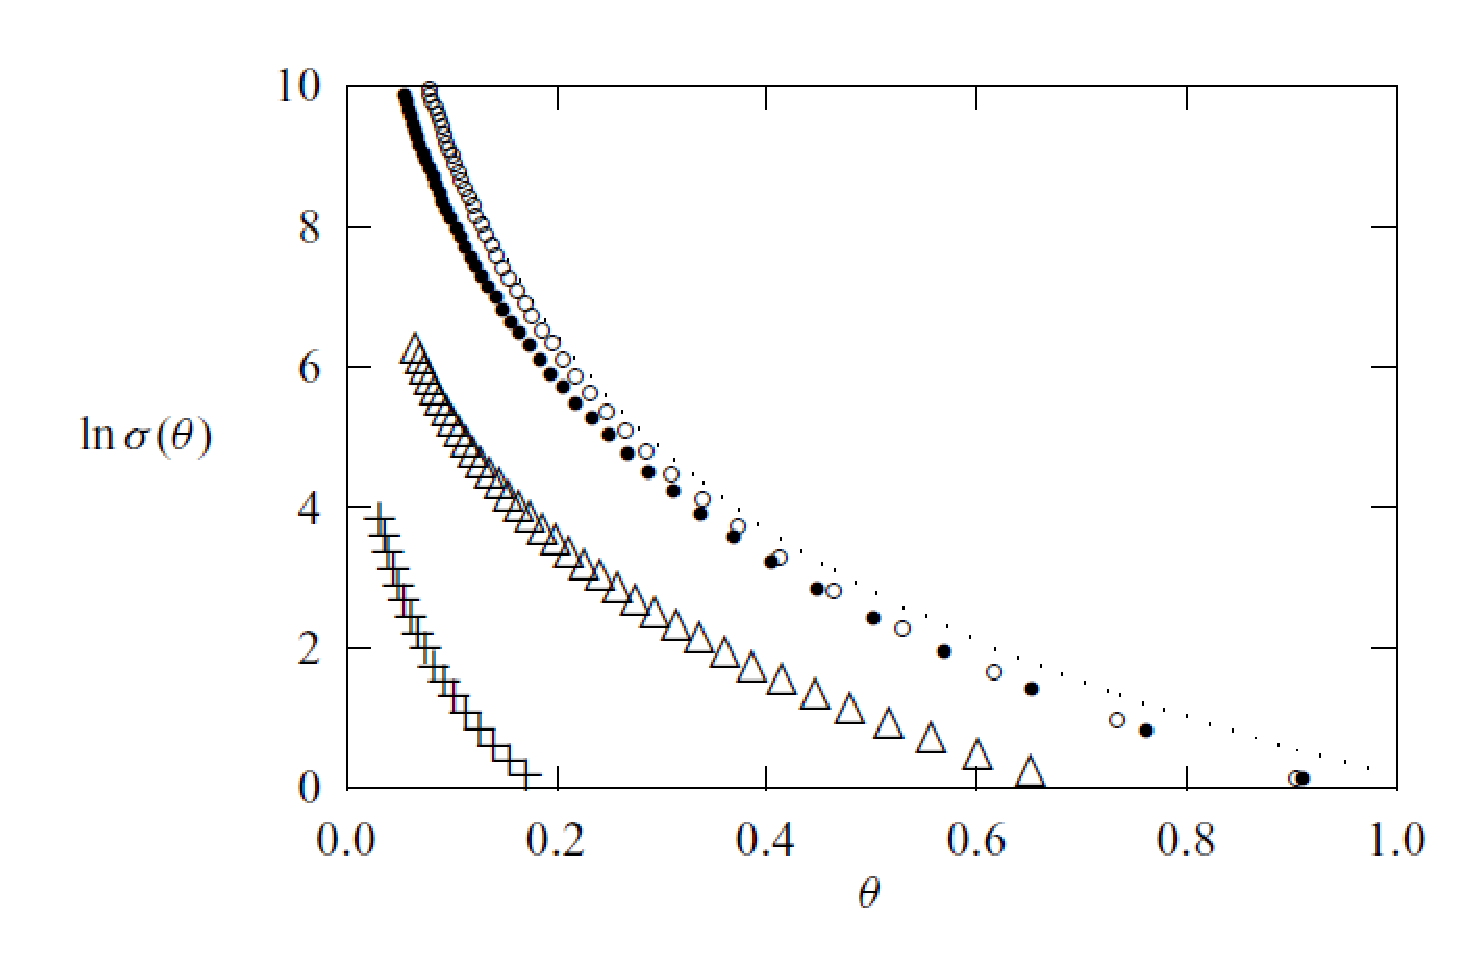
\includegraphics[scale=0.4]{Imagenes/graficadispersion_01.eps} 
\end{figure}
\end{frame}
% \begin{frame}
% \frametitle{Y para no aburrirse...}
% Podremos obtener entonces con todos los elementos señalados, una descripción de la dispersión clásica, y compararla con lo que ya sabemos de una dispersión con un potencial de tipo coulumbiano
% \[  V(r) = \dfrac{1}{4 \: \pi \: \epsilon_{0}} \; \dfrac{1}{r}\]
% \end{frame}
% \begin{frame}
% \frametitle{Y para no aburrirse...}
% Como un ejercicio para la tarea del tema, realizar el mismo procedimiento pero ahora con un potencial de tipo Lennard-Jones
% \[ V(r) = 4 \: \varepsilon \: \left[ \left( \dfrac{\sigma}{r} \right)^{12} - \left( \dfrac{\sigma}{r} \right)^{6} \right] \]
% \end{frame}
\end{document}